\documentclass[twoside]{book}

% Packages required by doxygen
\usepackage{fixltx2e}
\usepackage{calc}
\usepackage{doxygen}
\usepackage[export]{adjustbox} % also loads graphicx
\usepackage{graphicx}
\usepackage[utf8]{inputenc}
\usepackage{makeidx}
\usepackage{multicol}
\usepackage{multirow}
\PassOptionsToPackage{warn}{textcomp}
\usepackage{textcomp}
\usepackage[nointegrals]{wasysym}
\usepackage[table]{xcolor}

% Font selection
\usepackage[T1]{fontenc}
\usepackage[scaled=.90]{helvet}
\usepackage{courier}
\usepackage{amssymb}
\usepackage{sectsty}
\renewcommand{\familydefault}{\sfdefault}
\allsectionsfont{%
  \fontseries{bc}\selectfont%
  \color{darkgray}%
}
\renewcommand{\DoxyLabelFont}{%
  \fontseries{bc}\selectfont%
  \color{darkgray}%
}
\newcommand{\+}{\discretionary{\mbox{\scriptsize$\hookleftarrow$}}{}{}}

% Page & text layout
\usepackage{geometry}
\geometry{%
  a4paper,%
  top=2.5cm,%
  bottom=2.5cm,%
  left=2.5cm,%
  right=2.5cm%
}
\tolerance=750
\hfuzz=15pt
\hbadness=750
\setlength{\emergencystretch}{15pt}
\setlength{\parindent}{0cm}
\setlength{\parskip}{3ex plus 2ex minus 2ex}
\makeatletter
\renewcommand{\paragraph}{%
  \@startsection{paragraph}{4}{0ex}{-1.0ex}{1.0ex}{%
    \normalfont\normalsize\bfseries\SS@parafont%
  }%
}
\renewcommand{\subparagraph}{%
  \@startsection{subparagraph}{5}{0ex}{-1.0ex}{1.0ex}{%
    \normalfont\normalsize\bfseries\SS@subparafont%
  }%
}
\makeatother

% Headers & footers
\usepackage{fancyhdr}
\pagestyle{fancyplain}
\fancyhead[LE]{\fancyplain{}{\bfseries\thepage}}
\fancyhead[CE]{\fancyplain{}{}}
\fancyhead[RE]{\fancyplain{}{\bfseries\leftmark}}
\fancyhead[LO]{\fancyplain{}{\bfseries\rightmark}}
\fancyhead[CO]{\fancyplain{}{}}
\fancyhead[RO]{\fancyplain{}{\bfseries\thepage}}
\fancyfoot[LE]{\fancyplain{}{}}
\fancyfoot[CE]{\fancyplain{}{}}
\fancyfoot[RE]{\fancyplain{}{\bfseries\scriptsize Generated by Doxygen }}
\fancyfoot[LO]{\fancyplain{}{\bfseries\scriptsize Generated by Doxygen }}
\fancyfoot[CO]{\fancyplain{}{}}
\fancyfoot[RO]{\fancyplain{}{}}
\renewcommand{\footrulewidth}{0.4pt}
\renewcommand{\chaptermark}[1]{%
  \markboth{#1}{}%
}
\renewcommand{\sectionmark}[1]{%
  \markright{\thesection\ #1}%
}

% Indices & bibliography
\usepackage{natbib}
\usepackage[titles]{tocloft}
\setcounter{tocdepth}{3}
\setcounter{secnumdepth}{5}
\makeindex

% Hyperlinks (required, but should be loaded last)
\usepackage{ifpdf}
\ifpdf
  \usepackage[pdftex,pagebackref=true]{hyperref}
\else
  \usepackage[ps2pdf,pagebackref=true]{hyperref}
\fi
\hypersetup{%
  colorlinks=true,%
  linkcolor=blue,%
  citecolor=blue,%
  unicode%
}

% Custom commands
\newcommand{\clearemptydoublepage}{%
  \newpage{\pagestyle{empty}\cleardoublepage}%
}

\usepackage{caption}
\captionsetup{labelsep=space,justification=centering,font={bf},singlelinecheck=off,skip=4pt,position=top}

%===== C O N T E N T S =====

\begin{document}

% Titlepage & ToC
\hypersetup{pageanchor=false,
             bookmarksnumbered=true,
             pdfencoding=unicode
            }
\pagenumbering{roman}
\begin{titlepage}
\vspace*{7cm}
\begin{center}%
{\Large Remote Memory \\[1ex]\large 1.\+0.\+0v }\\
\vspace*{1cm}
{\large Generated by Doxygen 1.8.11}\\
\end{center}
\end{titlepage}
\clearemptydoublepage
\tableofcontents
\clearemptydoublepage
\pagenumbering{arabic}
\hypersetup{pageanchor=true}

%--- Begin generated contents ---
\chapter{Hierarchical Index}
\section{Jerarquía de la clase}
Esta lista de herencias esta ordenada aproximadamente por orden alfabético\+:\begin{DoxyCompactList}
\item Q\+Main\+Window\begin{DoxyCompactList}
\item \contentsline{section}{Main\+Window}{\pageref{classMainWindow}}{}
\end{DoxyCompactList}
\item Q\+Object\begin{DoxyCompactList}
\item \contentsline{section}{Socket\+Cliente}{\pageref{classSocketCliente}}{}
\end{DoxyCompactList}
\end{DoxyCompactList}

\chapter{Class Index}
\section{Lista de clases}
Lista de las clases, estructuras, uniones e interfaces con una breve descripción\+:\begin{DoxyCompactList}
\item\contentsline{section}{\hyperlink{classMainWindow}{Main\+Window} \\*The \hyperlink{classMainWindow}{Main\+Window} class }{\pageref{classMainWindow}}{}
\item\contentsline{section}{\hyperlink{classSocketCliente}{Socket\+Cliente} \\*The \hyperlink{classSocketCliente}{Socket\+Cliente} class }{\pageref{classSocketCliente}}{}
\end{DoxyCompactList}

\chapter{File Index}
\section{Lista de archivos}
Lista de todos los archivos documentados y con descripciones breves\+:\begin{DoxyCompactList}
\item\contentsline{section}{\hyperlink{mainwindow_8h}{mainwindow.\+h} \\*\hyperlink{classMainWindow}{Main\+Window} header }{\pageref{mainwindow_8h}}{}
\item\contentsline{section}{\hyperlink{socketcliente_8h}{socketcliente.\+h} \\*Contains a set of methods for handling Socket connection }{\pageref{socketcliente_8h}}{}
\end{DoxyCompactList}

\chapter{Class Documentation}
\hypertarget{classCache}{}\section{Cache Class Reference}
\label{classCache}\index{Cache@{Cache}}


The \hyperlink{classCache}{Cache} class.  




{\ttfamily \#include $<$cache.\+h$>$}

\subsection*{Public Member Functions}
\begin{DoxyCompactItemize}
\item 
\hyperlink{classCache_a486f257a48e32d0083f8ae41f78074d1}{Cache} ()\hypertarget{classCache_a486f257a48e32d0083f8ae41f78074d1}{}\label{classCache_a486f257a48e32d0083f8ae41f78074d1}

\begin{DoxyCompactList}\small\item\em Constructor. \end{DoxyCompactList}\item 
\hyperlink{classCache_af8b171a6c49d88d3ba179477484b9d48}{$\sim$\+Cache} ()\hypertarget{classCache_af8b171a6c49d88d3ba179477484b9d48}{}\label{classCache_af8b171a6c49d88d3ba179477484b9d48}

\begin{DoxyCompactList}\small\item\em Destructor. \end{DoxyCompactList}\item 
void \hyperlink{classCache_a424082d73c3ce7e78fb9d122c1a826c8}{add} (string data, string key)
\begin{DoxyCompactList}\small\item\em Appends the specified node to the end of this cache. \end{DoxyCompactList}\item 
bool \hyperlink{classCache_a868817da5b0a1a877b1b090a292b2175}{exist} (string key)
\begin{DoxyCompactList}\small\item\em Verify if the key is in cache. \end{DoxyCompactList}\item 
\hyperlink{classNodeCache}{Node\+Cache} $\ast$ \hyperlink{classCache_a5c64b3fb5b170fb15e94295a9a3668f9}{get} (int index)
\begin{DoxyCompactList}\small\item\em Returns the node at the specified position in this cache. \end{DoxyCompactList}\item 
\hyperlink{classNodeCache}{Node\+Cache} $\ast$ \hyperlink{classCache_a31cbe65db89b7840d8baa1baeb3b5c39}{get} (string key)
\begin{DoxyCompactList}\small\item\em Returns the node with the specified key in this cache. \end{DoxyCompactList}\item 
int \hyperlink{classCache_a1cf0dcb3da4880aa34ecbcfaaaccff52}{get\+\_\+size} ()
\begin{DoxyCompactList}\small\item\em Returns the number of nodes in this cache. \end{DoxyCompactList}\item 
void \hyperlink{classCache_a46fc7cbf5d26176b8c4b98adf96c6c25}{remove} (string key)
\begin{DoxyCompactList}\small\item\em Removes the node with the specified key in this cache. \end{DoxyCompactList}\item 
void \hyperlink{classCache_a171169132c9a4383f87c31ae146bf51b}{remove\+\_\+unless} ()\hypertarget{classCache_a171169132c9a4383f87c31ae146bf51b}{}\label{classCache_a171169132c9a4383f87c31ae146bf51b}

\begin{DoxyCompactList}\small\item\em Remove the least referenced node. \end{DoxyCompactList}\item 
\hyperlink{classNodeCache}{Node\+Cache} $\ast$ \hyperlink{classCache_a45fe41e77291379c0695ccfbd78fc967}{operator\mbox{[}$\,$\mbox{]}} (int index)
\begin{DoxyCompactList}\small\item\em operator \mbox{[}\mbox{]} \end{DoxyCompactList}\item 
\hyperlink{classNodeCache}{Node\+Cache} $\ast$ \hyperlink{classCache_aefeeb5ee4cdf8ad8c831b3c9edda52a0}{operator\mbox{[}$\,$\mbox{]}} (string key)
\begin{DoxyCompactList}\small\item\em Overload of the subscript operator. \end{DoxyCompactList}\end{DoxyCompactItemize}


\subsection{Detailed Description}
The \hyperlink{classCache}{Cache} class. 

\subsection{Member Function Documentation}
\index{Cache@{Cache}!add@{add}}
\index{add@{add}!Cache@{Cache}}
\subsubsection[{\texorpdfstring{add(string data, string key)}{add(string data, string key)}}]{\setlength{\rightskip}{0pt plus 5cm}void Cache\+::add (
\begin{DoxyParamCaption}
\item[{string}]{data, }
\item[{string}]{key}
\end{DoxyParamCaption}
)}\hypertarget{classCache_a424082d73c3ce7e78fb9d122c1a826c8}{}\label{classCache_a424082d73c3ce7e78fb9d122c1a826c8}


Appends the specified node to the end of this cache. 


\begin{DoxyExceptions}{Exceptions}
{\em string} & -\/ if the key already exists. \\
\hline
\end{DoxyExceptions}

\begin{DoxyParams}{Parameters}
{\em data} & -\/ data to store. \\
\hline
{\em key} & -\/ key as identifier of node. \\
\hline
\end{DoxyParams}
\index{Cache@{Cache}!exist@{exist}}
\index{exist@{exist}!Cache@{Cache}}
\subsubsection[{\texorpdfstring{exist(string key)}{exist(string key)}}]{\setlength{\rightskip}{0pt plus 5cm}bool Cache\+::exist (
\begin{DoxyParamCaption}
\item[{string}]{key}
\end{DoxyParamCaption}
)}\hypertarget{classCache_a868817da5b0a1a877b1b090a292b2175}{}\label{classCache_a868817da5b0a1a877b1b090a292b2175}


Verify if the key is in cache. 


\begin{DoxyParams}{Parameters}
{\em key} & -\/ key as identifier of node. \\
\hline
\end{DoxyParams}
\begin{DoxyReturn}{Returns}
true or false 
\end{DoxyReturn}
\index{Cache@{Cache}!get@{get}}
\index{get@{get}!Cache@{Cache}}
\subsubsection[{\texorpdfstring{get(int index)}{get(int index)}}]{\setlength{\rightskip}{0pt plus 5cm}{\bf Node\+Cache} $\ast$ Cache\+::get (
\begin{DoxyParamCaption}
\item[{int}]{index}
\end{DoxyParamCaption}
)}\hypertarget{classCache_a5c64b3fb5b170fb15e94295a9a3668f9}{}\label{classCache_a5c64b3fb5b170fb15e94295a9a3668f9}


Returns the node at the specified position in this cache. 


\begin{DoxyExceptions}{Exceptions}
{\em out\+\_\+of\+\_\+range} & -\/ if the index is out of range (index $<$ 0 $\vert$$\vert$ index $>$= size()). \\
\hline
\end{DoxyExceptions}

\begin{DoxyParams}{Parameters}
{\em index} & -\/ index of the node to return. \\
\hline
\end{DoxyParams}
\begin{DoxyReturn}{Returns}
the node at the specified position in this cache. 
\end{DoxyReturn}
\index{Cache@{Cache}!get@{get}}
\index{get@{get}!Cache@{Cache}}
\subsubsection[{\texorpdfstring{get(string key)}{get(string key)}}]{\setlength{\rightskip}{0pt plus 5cm}{\bf Node\+Cache} $\ast$ Cache\+::get (
\begin{DoxyParamCaption}
\item[{string}]{key}
\end{DoxyParamCaption}
)}\hypertarget{classCache_a31cbe65db89b7840d8baa1baeb3b5c39}{}\label{classCache_a31cbe65db89b7840d8baa1baeb3b5c39}


Returns the node with the specified key in this cache. 


\begin{DoxyExceptions}{Exceptions}
{\em exception} & -\/ if the key is not found. \\
\hline
\end{DoxyExceptions}

\begin{DoxyParams}{Parameters}
{\em key} & -\/ key of the node to search for. \\
\hline
\end{DoxyParams}
\begin{DoxyReturn}{Returns}
the node with the specified key in this cache. 
\end{DoxyReturn}
\index{Cache@{Cache}!get\+\_\+size@{get\+\_\+size}}
\index{get\+\_\+size@{get\+\_\+size}!Cache@{Cache}}
\subsubsection[{\texorpdfstring{get\+\_\+size()}{get_size()}}]{\setlength{\rightskip}{0pt plus 5cm}int Cache\+::get\+\_\+size (
\begin{DoxyParamCaption}
{}
\end{DoxyParamCaption}
)}\hypertarget{classCache_a1cf0dcb3da4880aa34ecbcfaaaccff52}{}\label{classCache_a1cf0dcb3da4880aa34ecbcfaaaccff52}


Returns the number of nodes in this cache. 

\begin{DoxyReturn}{Returns}
the number of nodes in this cache. 
\end{DoxyReturn}
\index{Cache@{Cache}!operator\mbox{[}$\,$\mbox{]}@{operator[]}}
\index{operator\mbox{[}$\,$\mbox{]}@{operator[]}!Cache@{Cache}}
\subsubsection[{\texorpdfstring{operator[](int index)}{operator[](int index)}}]{\setlength{\rightskip}{0pt plus 5cm}{\bf Node\+Cache}$\ast$ Cache\+::operator\mbox{[}$\,$\mbox{]} (
\begin{DoxyParamCaption}
\item[{int}]{index}
\end{DoxyParamCaption}
)\hspace{0.3cm}{\ttfamily [inline]}}\hypertarget{classCache_a45fe41e77291379c0695ccfbd78fc967}{}\label{classCache_a45fe41e77291379c0695ccfbd78fc967}


operator \mbox{[}\mbox{]} 


\begin{DoxyExceptions}{Exceptions}
{\em out\+\_\+of\+\_\+range} & -\/ if the index is out of range (index $<$ 0 $\vert$$\vert$ index $>$= size()). \\
\hline
\end{DoxyExceptions}

\begin{DoxyParams}{Parameters}
{\em index} & -\/ index of the node to return. \\
\hline
\end{DoxyParams}
\begin{DoxyReturn}{Returns}
the node at the specified position in this cache. 
\end{DoxyReturn}
\index{Cache@{Cache}!operator\mbox{[}$\,$\mbox{]}@{operator[]}}
\index{operator\mbox{[}$\,$\mbox{]}@{operator[]}!Cache@{Cache}}
\subsubsection[{\texorpdfstring{operator[](string key)}{operator[](string key)}}]{\setlength{\rightskip}{0pt plus 5cm}{\bf Node\+Cache}$\ast$ Cache\+::operator\mbox{[}$\,$\mbox{]} (
\begin{DoxyParamCaption}
\item[{string}]{key}
\end{DoxyParamCaption}
)\hspace{0.3cm}{\ttfamily [inline]}}\hypertarget{classCache_aefeeb5ee4cdf8ad8c831b3c9edda52a0}{}\label{classCache_aefeeb5ee4cdf8ad8c831b3c9edda52a0}


Overload of the subscript operator. 


\begin{DoxyExceptions}{Exceptions}
{\em exception} & -\/ if the key is not found. \\
\hline
\end{DoxyExceptions}

\begin{DoxyParams}{Parameters}
{\em key} & -\/ key of the node to search for. \\
\hline
\end{DoxyParams}
\begin{DoxyReturn}{Returns}
the node with the specified key in this cache. 
\end{DoxyReturn}
\index{Cache@{Cache}!remove@{remove}}
\index{remove@{remove}!Cache@{Cache}}
\subsubsection[{\texorpdfstring{remove(string key)}{remove(string key)}}]{\setlength{\rightskip}{0pt plus 5cm}void Cache\+::remove (
\begin{DoxyParamCaption}
\item[{string}]{key}
\end{DoxyParamCaption}
)}\hypertarget{classCache_a46fc7cbf5d26176b8c4b98adf96c6c25}{}\label{classCache_a46fc7cbf5d26176b8c4b98adf96c6c25}


Removes the node with the specified key in this cache. 


\begin{DoxyExceptions}{Exceptions}
{\em exception} & -\/ if the key is not found. \\
\hline
\end{DoxyExceptions}

\begin{DoxyParams}{Parameters}
{\em key} & -\/ key of the node to remove for. \\
\hline
\end{DoxyParams}


The documentation for this class was generated from the following files\+:\begin{DoxyCompactItemize}
\item 
\hyperlink{cache_8h}{cache.\+h}\item 
cache.\+cpp\end{DoxyCompactItemize}

\hypertarget{structDataSocket}{}\section{Data\+Socket Struct Reference}
\label{structDataSocket}\index{Data\+Socket@{Data\+Socket}}


The \hyperlink{structDataSocket}{Data\+Socket} struct.  




{\ttfamily \#include $<$socketserver.\+h$>$}

\subsection*{Public Attributes}
\begin{DoxyCompactItemize}
\item 
int \hyperlink{structDataSocket_a36208fdb5bdecfb536f2b216f31c6a90}{descriptor}\hypertarget{structDataSocket_a36208fdb5bdecfb536f2b216f31c6a90}{}\label{structDataSocket_a36208fdb5bdecfb536f2b216f31c6a90}

\begin{DoxyCompactList}\small\item\em identifier. \end{DoxyCompactList}\item 
sockaddr\+\_\+in \hyperlink{structDataSocket_a68cf3c516272641695f0272ab5f33c78}{info}\hypertarget{structDataSocket_a68cf3c516272641695f0272ab5f33c78}{}\label{structDataSocket_a68cf3c516272641695f0272ab5f33c78}

\begin{DoxyCompactList}\small\item\em information. \end{DoxyCompactList}\end{DoxyCompactItemize}


\subsection{Detailed Description}
The \hyperlink{structDataSocket}{Data\+Socket} struct. 

The documentation for this struct was generated from the following file\+:\begin{DoxyCompactItemize}
\item 
socketserver.\+h\end{DoxyCompactItemize}

\hypertarget{classMainWindow}{}\section{Referencia de la Clase Main\+Window}
\label{classMainWindow}\index{Main\+Window@{Main\+Window}}


The \hyperlink{classMainWindow}{Main\+Window} class.  




{\ttfamily \#include $<$mainwindow.\+h$>$}



Diagrama de herencias de Main\+Window
\nopagebreak
\begin{figure}[H]
\begin{center}
\leavevmode
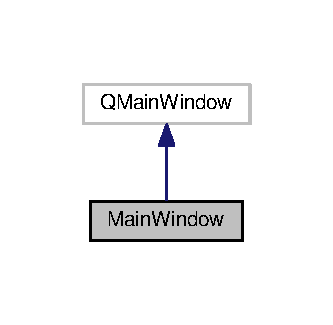
\includegraphics[width=160pt]{classMainWindow__inherit__graph}
\end{center}
\end{figure}


Diagrama de colaboración para Main\+Window\+:
\nopagebreak
\begin{figure}[H]
\begin{center}
\leavevmode
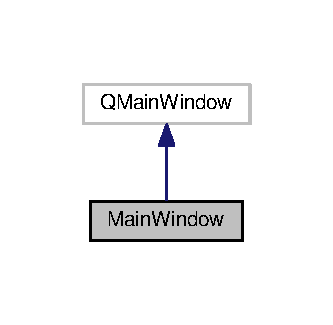
\includegraphics[width=160pt]{classMainWindow__coll__graph}
\end{center}
\end{figure}
\subsection*{Métodos públicos}
\begin{DoxyCompactItemize}
\item 
\hyperlink{classMainWindow_a8b244be8b7b7db1b08de2a2acb9409db}{Main\+Window} (Q\+Widget $\ast$parent=0)
\begin{DoxyCompactList}\small\item\em Constructor. \end{DoxyCompactList}\item 
\hyperlink{classMainWindow_ae98d00a93bc118200eeef9f9bba1dba7}{$\sim$\+Main\+Window} ()\hypertarget{classMainWindow_ae98d00a93bc118200eeef9f9bba1dba7}{}\label{classMainWindow_ae98d00a93bc118200eeef9f9bba1dba7}

\begin{DoxyCompactList}\small\item\em Destructor. \end{DoxyCompactList}\end{DoxyCompactItemize}


\subsection{Descripción detallada}
The \hyperlink{classMainWindow}{Main\+Window} class. 

\subsection{Documentación del constructor y destructor}
\index{Main\+Window@{Main\+Window}!Main\+Window@{Main\+Window}}
\index{Main\+Window@{Main\+Window}!Main\+Window@{Main\+Window}}
\subsubsection[{\texorpdfstring{Main\+Window(\+Q\+Widget $\ast$parent=0)}{MainWindow(QWidget *parent=0)}}]{\setlength{\rightskip}{0pt plus 5cm}Main\+Window\+::\+Main\+Window (
\begin{DoxyParamCaption}
\item[{Q\+Widget $\ast$}]{parent = {\ttfamily 0}}
\end{DoxyParamCaption}
)\hspace{0.3cm}{\ttfamily [explicit]}}\hypertarget{classMainWindow_a8b244be8b7b7db1b08de2a2acb9409db}{}\label{classMainWindow_a8b244be8b7b7db1b08de2a2acb9409db}


Constructor. 


\begin{DoxyParams}{Parámetros}
{\em parent} & -\/ pointer of Q\+Widget object. \\
\hline
\end{DoxyParams}


La documentación para esta clase fue generada a partir de los siguientes ficheros\+:\begin{DoxyCompactItemize}
\item 
\hyperlink{mainwindow_8h}{mainwindow.\+h}\item 
mainwindow.\+cpp\end{DoxyCompactItemize}

\hypertarget{classMemory}{}\section{Memory Class Reference}
\label{classMemory}\index{Memory@{Memory}}


The \hyperlink{classMemory}{Memory} class.  




{\ttfamily \#include $<$memory.\+h$>$}

\subsection*{Public Member Functions}
\begin{DoxyCompactItemize}
\item 
\hyperlink{classMemory_a585d7bb6fc6f2237bcebf94a86b7dd99}{Memory} ()\hypertarget{classMemory_a585d7bb6fc6f2237bcebf94a86b7dd99}{}\label{classMemory_a585d7bb6fc6f2237bcebf94a86b7dd99}

\begin{DoxyCompactList}\small\item\em Constructor. \end{DoxyCompactList}\item 
\hyperlink{classMemory_a0ffa9759ebbf103f11132a505b93bdc0}{$\sim$\+Memory} ()\hypertarget{classMemory_a0ffa9759ebbf103f11132a505b93bdc0}{}\label{classMemory_a0ffa9759ebbf103f11132a505b93bdc0}

\begin{DoxyCompactList}\small\item\em Destructor. \end{DoxyCompactList}\item 
void \hyperlink{classMemory_a1c5845ec12edc89a46ae9a429751dad4}{add} (string data, string key)
\begin{DoxyCompactList}\small\item\em Appends the specified node to the end of this list. \end{DoxyCompactList}\item 
bool \hyperlink{classMemory_ab7f1b528e6d338a6e8a34213e84428f8}{exist} (string key)
\begin{DoxyCompactList}\small\item\em Verify if the key is this list. \end{DoxyCompactList}\item 
\hyperlink{classNodeMemory}{Node\+Memory} $\ast$ \hyperlink{classMemory_abad3ec0c9cd654bed7dbbc94f84d7109}{get} (int index)
\begin{DoxyCompactList}\small\item\em Returns the node at the specified position in this list. \end{DoxyCompactList}\item 
\hyperlink{classNodeMemory}{Node\+Memory} $\ast$ \hyperlink{classMemory_a4e46131b5a3dbf96258d7c5ebe665f32}{get} (string key)
\begin{DoxyCompactList}\small\item\em Returns the node with the specified key in this list. \end{DoxyCompactList}\item 
int \hyperlink{classMemory_a1c3e9773bfe8ca3f70cfdfd1400b5851}{get\+\_\+size} ()
\begin{DoxyCompactList}\small\item\em Returns the number of elements in this list. \end{DoxyCompactList}\item 
void \hyperlink{classMemory_a75a4c6877d75391b28778671cbd523b4}{remove} (int index)
\begin{DoxyCompactList}\small\item\em Removes the element at the specified position in this list. \end{DoxyCompactList}\item 
void \hyperlink{classMemory_a3a048dda4d162dcd396bcc2e1f454bfb}{remove} (string key)
\begin{DoxyCompactList}\small\item\em Removes the element witht the specified key in this list. \end{DoxyCompactList}\item 
\hyperlink{classNodeMemory}{Node\+Memory} $\ast$ \hyperlink{classMemory_a1a56f0b08a50f64a526b8a0712ea8f5f}{operator\mbox{[}$\,$\mbox{]}} (int index)
\begin{DoxyCompactList}\small\item\em operator \mbox{[}\mbox{]} \end{DoxyCompactList}\item 
\hyperlink{classNodeMemory}{Node\+Memory} $\ast$ \hyperlink{classMemory_a5bd91f228b80bfd56b3bf82ebc16f41f}{operator\mbox{[}$\,$\mbox{]}} (string key)
\begin{DoxyCompactList}\small\item\em Overload of the subscript operator. \end{DoxyCompactList}\end{DoxyCompactItemize}


\subsection{Detailed Description}
The \hyperlink{classMemory}{Memory} class. 

\subsection{Member Function Documentation}
\index{Memory@{Memory}!add@{add}}
\index{add@{add}!Memory@{Memory}}
\subsubsection[{\texorpdfstring{add(string data, string key)}{add(string data, string key)}}]{\setlength{\rightskip}{0pt plus 5cm}void Memory\+::add (
\begin{DoxyParamCaption}
\item[{string}]{data, }
\item[{string}]{key}
\end{DoxyParamCaption}
)}\hypertarget{classMemory_a1c5845ec12edc89a46ae9a429751dad4}{}\label{classMemory_a1c5845ec12edc89a46ae9a429751dad4}


Appends the specified node to the end of this list. 


\begin{DoxyExceptions}{Exceptions}
{\em string} & -\/ if the key already exists. \\
\hline
\end{DoxyExceptions}

\begin{DoxyParams}{Parameters}
{\em data} & -\/ data to store. \\
\hline
{\em key} & -\/ key as identifier of node. \\
\hline
\end{DoxyParams}
\index{Memory@{Memory}!exist@{exist}}
\index{exist@{exist}!Memory@{Memory}}
\subsubsection[{\texorpdfstring{exist(string key)}{exist(string key)}}]{\setlength{\rightskip}{0pt plus 5cm}bool Memory\+::exist (
\begin{DoxyParamCaption}
\item[{string}]{key}
\end{DoxyParamCaption}
)}\hypertarget{classMemory_ab7f1b528e6d338a6e8a34213e84428f8}{}\label{classMemory_ab7f1b528e6d338a6e8a34213e84428f8}


Verify if the key is this list. 


\begin{DoxyParams}{Parameters}
{\em key} & -\/ key as identifier of node. \\
\hline
\end{DoxyParams}
\begin{DoxyReturn}{Returns}
true or false 
\end{DoxyReturn}
\index{Memory@{Memory}!get@{get}}
\index{get@{get}!Memory@{Memory}}
\subsubsection[{\texorpdfstring{get(int index)}{get(int index)}}]{\setlength{\rightskip}{0pt plus 5cm}{\bf Node\+Memory} $\ast$ Memory\+::get (
\begin{DoxyParamCaption}
\item[{int}]{index}
\end{DoxyParamCaption}
)}\hypertarget{classMemory_abad3ec0c9cd654bed7dbbc94f84d7109}{}\label{classMemory_abad3ec0c9cd654bed7dbbc94f84d7109}


Returns the node at the specified position in this list. 


\begin{DoxyExceptions}{Exceptions}
{\em out\+\_\+of\+\_\+range} & -\/ if the index is out of range (index $<$ 0 $\vert$$\vert$ index $>$= size()). \\
\hline
\end{DoxyExceptions}

\begin{DoxyParams}{Parameters}
{\em index} & -\/ index of the node to return. \\
\hline
\end{DoxyParams}
\begin{DoxyReturn}{Returns}
the node at the specified position in this list. 
\end{DoxyReturn}
\index{Memory@{Memory}!get@{get}}
\index{get@{get}!Memory@{Memory}}
\subsubsection[{\texorpdfstring{get(string key)}{get(string key)}}]{\setlength{\rightskip}{0pt plus 5cm}{\bf Node\+Memory} $\ast$ Memory\+::get (
\begin{DoxyParamCaption}
\item[{string}]{key}
\end{DoxyParamCaption}
)}\hypertarget{classMemory_a4e46131b5a3dbf96258d7c5ebe665f32}{}\label{classMemory_a4e46131b5a3dbf96258d7c5ebe665f32}


Returns the node with the specified key in this list. 


\begin{DoxyExceptions}{Exceptions}
{\em exception} & -\/ if the key is not found. \\
\hline
\end{DoxyExceptions}

\begin{DoxyParams}{Parameters}
{\em key} & -\/ key of the node to search for. \\
\hline
\end{DoxyParams}
\begin{DoxyReturn}{Returns}
the node with the specified key in this list. 
\end{DoxyReturn}
\index{Memory@{Memory}!get\+\_\+size@{get\+\_\+size}}
\index{get\+\_\+size@{get\+\_\+size}!Memory@{Memory}}
\subsubsection[{\texorpdfstring{get\+\_\+size()}{get_size()}}]{\setlength{\rightskip}{0pt plus 5cm}int Memory\+::get\+\_\+size (
\begin{DoxyParamCaption}
{}
\end{DoxyParamCaption}
)}\hypertarget{classMemory_a1c3e9773bfe8ca3f70cfdfd1400b5851}{}\label{classMemory_a1c3e9773bfe8ca3f70cfdfd1400b5851}


Returns the number of elements in this list. 

\begin{DoxyReturn}{Returns}
the number of elements in this list. 
\end{DoxyReturn}
\index{Memory@{Memory}!operator\mbox{[}$\,$\mbox{]}@{operator[]}}
\index{operator\mbox{[}$\,$\mbox{]}@{operator[]}!Memory@{Memory}}
\subsubsection[{\texorpdfstring{operator[](int index)}{operator[](int index)}}]{\setlength{\rightskip}{0pt plus 5cm}{\bf Node\+Memory}$\ast$ Memory\+::operator\mbox{[}$\,$\mbox{]} (
\begin{DoxyParamCaption}
\item[{int}]{index}
\end{DoxyParamCaption}
)\hspace{0.3cm}{\ttfamily [inline]}}\hypertarget{classMemory_a1a56f0b08a50f64a526b8a0712ea8f5f}{}\label{classMemory_a1a56f0b08a50f64a526b8a0712ea8f5f}


operator \mbox{[}\mbox{]} 


\begin{DoxyExceptions}{Exceptions}
{\em out\+\_\+of\+\_\+range} & -\/ if the index is out of range (index $<$ 0 $\vert$$\vert$ index $>$= size()). \\
\hline
\end{DoxyExceptions}

\begin{DoxyParams}{Parameters}
{\em index} & -\/ index of the node to return. \\
\hline
\end{DoxyParams}
\begin{DoxyReturn}{Returns}
the node at the specified position in this cache. 
\end{DoxyReturn}
\index{Memory@{Memory}!operator\mbox{[}$\,$\mbox{]}@{operator[]}}
\index{operator\mbox{[}$\,$\mbox{]}@{operator[]}!Memory@{Memory}}
\subsubsection[{\texorpdfstring{operator[](string key)}{operator[](string key)}}]{\setlength{\rightskip}{0pt plus 5cm}{\bf Node\+Memory}$\ast$ Memory\+::operator\mbox{[}$\,$\mbox{]} (
\begin{DoxyParamCaption}
\item[{string}]{key}
\end{DoxyParamCaption}
)\hspace{0.3cm}{\ttfamily [inline]}}\hypertarget{classMemory_a5bd91f228b80bfd56b3bf82ebc16f41f}{}\label{classMemory_a5bd91f228b80bfd56b3bf82ebc16f41f}


Overload of the subscript operator. 


\begin{DoxyExceptions}{Exceptions}
{\em exception} & -\/ if the key is not found. \\
\hline
\end{DoxyExceptions}

\begin{DoxyParams}{Parameters}
{\em key} & -\/ key of the node to search for. \\
\hline
\end{DoxyParams}
\begin{DoxyReturn}{Returns}
the node with the specified key in this cache. 
\end{DoxyReturn}
\index{Memory@{Memory}!remove@{remove}}
\index{remove@{remove}!Memory@{Memory}}
\subsubsection[{\texorpdfstring{remove(int index)}{remove(int index)}}]{\setlength{\rightskip}{0pt plus 5cm}void Memory\+::remove (
\begin{DoxyParamCaption}
\item[{int}]{index}
\end{DoxyParamCaption}
)}\hypertarget{classMemory_a75a4c6877d75391b28778671cbd523b4}{}\label{classMemory_a75a4c6877d75391b28778671cbd523b4}


Removes the element at the specified position in this list. 


\begin{DoxyExceptions}{Exceptions}
{\em out\+\_\+of\+\_\+range} & -\/ if the index is out of range (index $<$ 0 $\vert$$\vert$ index $>$= size()). \\
\hline
\end{DoxyExceptions}

\begin{DoxyParams}{Parameters}
{\em index} & -\/ the index of the element to be removed. \\
\hline
\end{DoxyParams}
\index{Memory@{Memory}!remove@{remove}}
\index{remove@{remove}!Memory@{Memory}}
\subsubsection[{\texorpdfstring{remove(string key)}{remove(string key)}}]{\setlength{\rightskip}{0pt plus 5cm}void Memory\+::remove (
\begin{DoxyParamCaption}
\item[{string}]{key}
\end{DoxyParamCaption}
)}\hypertarget{classMemory_a3a048dda4d162dcd396bcc2e1f454bfb}{}\label{classMemory_a3a048dda4d162dcd396bcc2e1f454bfb}


Removes the element witht the specified key in this list. 


\begin{DoxyExceptions}{Exceptions}
{\em exception} & -\/ if the key is not found. \\
\hline
\end{DoxyExceptions}

\begin{DoxyParams}{Parameters}
{\em key} & -\/ key of the node to remove for. \\
\hline
\end{DoxyParams}


The documentation for this class was generated from the following files\+:\begin{DoxyCompactItemize}
\item 
memory.\+h\item 
memory.\+cpp\end{DoxyCompactItemize}

\hypertarget{classNodeCache}{}\section{Node\+Cache Class Reference}
\label{classNodeCache}\index{Node\+Cache@{Node\+Cache}}


The Node class.  




{\ttfamily \#include $<$nodecache.\+h$>$}

\subsection*{Public Member Functions}
\begin{DoxyCompactItemize}
\item 
void \hyperlink{classNodeCache_a7e621b939cdbc80967e6590b8ad86d73}{count\+\_\+accessed} ()\hypertarget{classNodeCache_a7e621b939cdbc80967e6590b8ad86d73}{}\label{classNodeCache_a7e621b939cdbc80967e6590b8ad86d73}

\begin{DoxyCompactList}\small\item\em Count a new access to this node. \end{DoxyCompactList}\item 
\hyperlink{classNodeCache_adec4f6cc00d2453f4da34c06e241d874}{Node\+Cache} (string data, string key)
\begin{DoxyCompactList}\small\item\em Constuctor. \end{DoxyCompactList}\item 
\hyperlink{classNodeCache_ad17fbdbc7a4fe97645919d7ebd88edbe}{$\sim$\+Node\+Cache} ()\hypertarget{classNodeCache_ad17fbdbc7a4fe97645919d7ebd88edbe}{}\label{classNodeCache_ad17fbdbc7a4fe97645919d7ebd88edbe}

\begin{DoxyCompactList}\small\item\em Destructor. \end{DoxyCompactList}\item 
int \hyperlink{classNodeCache_a78c4d4818132f8acace40f5c9a95a526}{get\+\_\+accessed} ()
\begin{DoxyCompactList}\small\item\em Return how many accessed have had this node. \end{DoxyCompactList}\item 
string \hyperlink{classNodeCache_ae11cea2fa334e2f653d46938ac4c97a8}{get\+\_\+data} ()
\begin{DoxyCompactList}\small\item\em Returns the data stores in this node. \end{DoxyCompactList}\item 
string \hyperlink{classNodeCache_a9d41e568632b7382a7f470c70c416028}{get\+\_\+key} ()
\begin{DoxyCompactList}\small\item\em Returns the key to identify this node. \end{DoxyCompactList}\item 
\hyperlink{classNodeCache}{Node\+Cache} $\ast$ \hyperlink{classNodeCache_a3c3e2abe476346e2f1ec31ea6fc31111}{get\+\_\+next} ()
\begin{DoxyCompactList}\small\item\em Returns a pointer to the next node. \end{DoxyCompactList}\item 
void \hyperlink{classNodeCache_aa83c8629d2b01dfaa0149a63d17c31e1}{set\+\_\+data} (string data)
\begin{DoxyCompactList}\small\item\em Set the new data to store in this node. \end{DoxyCompactList}\item 
void \hyperlink{classNodeCache_af45873de5ff6c83e3b9d92832dec2199}{set\+\_\+key} (string key)
\begin{DoxyCompactList}\small\item\em Set the new key to identify this node. \end{DoxyCompactList}\item 
void \hyperlink{classNodeCache_ad733051c05052913ec36c01e7bbc1332}{set\+\_\+next} (\hyperlink{classNodeCache}{Node\+Cache} $\ast$next)
\begin{DoxyCompactList}\small\item\em Set the new next node to this node. \end{DoxyCompactList}\item 
bool \hyperlink{classNodeCache_aaa1cb454234f2e2485ddcda0aff3585e}{operator==} (const \hyperlink{classNodeCache}{Node\+Cache} \&node)
\begin{DoxyCompactList}\small\item\em Overload of the comparison operator. Compare if two nodes are equal. \end{DoxyCompactList}\item 
bool \hyperlink{classNodeCache_a1f82522f7c1c6bac65472eba595ddaa7}{operator!=} (const \hyperlink{classNodeCache}{Node\+Cache} \&node)
\begin{DoxyCompactList}\small\item\em Overload of the different operator. Compare if two nodes are different. \end{DoxyCompactList}\item 
void \hyperlink{classNodeCache_aea15a590ffd1d581ce889e6117daac24}{operator=} (const \hyperlink{classNodeCache}{Node\+Cache} \&node)
\begin{DoxyCompactList}\small\item\em Copy the information from a node to other. \end{DoxyCompactList}\end{DoxyCompactItemize}
\subsection*{Friends}
\begin{DoxyCompactItemize}
\item 
ostream \& \hyperlink{classNodeCache_a2d3b986da4a23b4a456738290cc0b94e}{operator$<$$<$} (ostream \&output, const \hyperlink{classNodeCache}{Node\+Cache} \&node)
\begin{DoxyCompactList}\small\item\em Overload of the output operator. \end{DoxyCompactList}\end{DoxyCompactItemize}


\subsection{Detailed Description}
The Node class. 

\subsection{Constructor \& Destructor Documentation}
\index{Node\+Cache@{Node\+Cache}!Node\+Cache@{Node\+Cache}}
\index{Node\+Cache@{Node\+Cache}!Node\+Cache@{Node\+Cache}}
\subsubsection[{\texorpdfstring{Node\+Cache(string data, string key)}{NodeCache(string data, string key)}}]{\setlength{\rightskip}{0pt plus 5cm}Node\+Cache\+::\+Node\+Cache (
\begin{DoxyParamCaption}
\item[{string}]{data, }
\item[{string}]{key}
\end{DoxyParamCaption}
)}\hypertarget{classNodeCache_adec4f6cc00d2453f4da34c06e241d874}{}\label{classNodeCache_adec4f6cc00d2453f4da34c06e241d874}


Constuctor. 


\begin{DoxyParams}{Parameters}
{\em data} & -\/ data to store. \\
\hline
{\em key} & -\/ key to identify this node. \\
\hline
\end{DoxyParams}


\subsection{Member Function Documentation}
\index{Node\+Cache@{Node\+Cache}!get\+\_\+accessed@{get\+\_\+accessed}}
\index{get\+\_\+accessed@{get\+\_\+accessed}!Node\+Cache@{Node\+Cache}}
\subsubsection[{\texorpdfstring{get\+\_\+accessed()}{get_accessed()}}]{\setlength{\rightskip}{0pt plus 5cm}int Node\+Cache\+::get\+\_\+accessed (
\begin{DoxyParamCaption}
{}
\end{DoxyParamCaption}
)}\hypertarget{classNodeCache_a78c4d4818132f8acace40f5c9a95a526}{}\label{classNodeCache_a78c4d4818132f8acace40f5c9a95a526}


Return how many accessed have had this node. 

\begin{DoxyReturn}{Returns}
how many accessed have had this node. 
\end{DoxyReturn}
\index{Node\+Cache@{Node\+Cache}!get\+\_\+data@{get\+\_\+data}}
\index{get\+\_\+data@{get\+\_\+data}!Node\+Cache@{Node\+Cache}}
\subsubsection[{\texorpdfstring{get\+\_\+data()}{get_data()}}]{\setlength{\rightskip}{0pt plus 5cm}string Node\+Cache\+::get\+\_\+data (
\begin{DoxyParamCaption}
{}
\end{DoxyParamCaption}
)}\hypertarget{classNodeCache_ae11cea2fa334e2f653d46938ac4c97a8}{}\label{classNodeCache_ae11cea2fa334e2f653d46938ac4c97a8}


Returns the data stores in this node. 

\begin{DoxyReturn}{Returns}
data in this node. 
\end{DoxyReturn}
\index{Node\+Cache@{Node\+Cache}!get\+\_\+key@{get\+\_\+key}}
\index{get\+\_\+key@{get\+\_\+key}!Node\+Cache@{Node\+Cache}}
\subsubsection[{\texorpdfstring{get\+\_\+key()}{get_key()}}]{\setlength{\rightskip}{0pt plus 5cm}string Node\+Cache\+::get\+\_\+key (
\begin{DoxyParamCaption}
{}
\end{DoxyParamCaption}
)}\hypertarget{classNodeCache_a9d41e568632b7382a7f470c70c416028}{}\label{classNodeCache_a9d41e568632b7382a7f470c70c416028}


Returns the key to identify this node. 

\begin{DoxyReturn}{Returns}
key to identify this node. 
\end{DoxyReturn}
\index{Node\+Cache@{Node\+Cache}!get\+\_\+next@{get\+\_\+next}}
\index{get\+\_\+next@{get\+\_\+next}!Node\+Cache@{Node\+Cache}}
\subsubsection[{\texorpdfstring{get\+\_\+next()}{get_next()}}]{\setlength{\rightskip}{0pt plus 5cm}{\bf Node\+Cache} $\ast$ Node\+Cache\+::get\+\_\+next (
\begin{DoxyParamCaption}
{}
\end{DoxyParamCaption}
)}\hypertarget{classNodeCache_a3c3e2abe476346e2f1ec31ea6fc31111}{}\label{classNodeCache_a3c3e2abe476346e2f1ec31ea6fc31111}


Returns a pointer to the next node. 

\begin{DoxyReturn}{Returns}
pointer to the next node. 
\end{DoxyReturn}
\index{Node\+Cache@{Node\+Cache}!operator"!=@{operator"!=}}
\index{operator"!=@{operator"!=}!Node\+Cache@{Node\+Cache}}
\subsubsection[{\texorpdfstring{operator"!=(const Node\+Cache \&node)}{operator!=(const NodeCache &node)}}]{\setlength{\rightskip}{0pt plus 5cm}bool Node\+Cache\+::operator!= (
\begin{DoxyParamCaption}
\item[{const {\bf Node\+Cache} \&}]{node}
\end{DoxyParamCaption}
)\hspace{0.3cm}{\ttfamily [inline]}}\hypertarget{classNodeCache_a1f82522f7c1c6bac65472eba595ddaa7}{}\label{classNodeCache_a1f82522f7c1c6bac65472eba595ddaa7}


Overload of the different operator. Compare if two nodes are different. 


\begin{DoxyParams}{Parameters}
{\em node} & -\/ node wich it is compared. \\
\hline
\end{DoxyParams}
\begin{DoxyReturn}{Returns}
true or false. 
\end{DoxyReturn}
\index{Node\+Cache@{Node\+Cache}!operator=@{operator=}}
\index{operator=@{operator=}!Node\+Cache@{Node\+Cache}}
\subsubsection[{\texorpdfstring{operator=(const Node\+Cache \&node)}{operator=(const NodeCache &node)}}]{\setlength{\rightskip}{0pt plus 5cm}void Node\+Cache\+::operator= (
\begin{DoxyParamCaption}
\item[{const {\bf Node\+Cache} \&}]{node}
\end{DoxyParamCaption}
)\hspace{0.3cm}{\ttfamily [inline]}}\hypertarget{classNodeCache_aea15a590ffd1d581ce889e6117daac24}{}\label{classNodeCache_aea15a590ffd1d581ce889e6117daac24}


Copy the information from a node to other. 


\begin{DoxyParams}{Parameters}
{\em node} & -\/ node with the information to copy. \\
\hline
\end{DoxyParams}
\index{Node\+Cache@{Node\+Cache}!operator==@{operator==}}
\index{operator==@{operator==}!Node\+Cache@{Node\+Cache}}
\subsubsection[{\texorpdfstring{operator==(const Node\+Cache \&node)}{operator==(const NodeCache &node)}}]{\setlength{\rightskip}{0pt plus 5cm}bool Node\+Cache\+::operator== (
\begin{DoxyParamCaption}
\item[{const {\bf Node\+Cache} \&}]{node}
\end{DoxyParamCaption}
)\hspace{0.3cm}{\ttfamily [inline]}}\hypertarget{classNodeCache_aaa1cb454234f2e2485ddcda0aff3585e}{}\label{classNodeCache_aaa1cb454234f2e2485ddcda0aff3585e}


Overload of the comparison operator. Compare if two nodes are equal. 


\begin{DoxyParams}{Parameters}
{\em node} & -\/ node wich it is compared. \\
\hline
\end{DoxyParams}
\begin{DoxyReturn}{Returns}
true or false. 
\end{DoxyReturn}
\index{Node\+Cache@{Node\+Cache}!set\+\_\+data@{set\+\_\+data}}
\index{set\+\_\+data@{set\+\_\+data}!Node\+Cache@{Node\+Cache}}
\subsubsection[{\texorpdfstring{set\+\_\+data(string data)}{set_data(string data)}}]{\setlength{\rightskip}{0pt plus 5cm}void Node\+Cache\+::set\+\_\+data (
\begin{DoxyParamCaption}
\item[{string}]{data}
\end{DoxyParamCaption}
)}\hypertarget{classNodeCache_aa83c8629d2b01dfaa0149a63d17c31e1}{}\label{classNodeCache_aa83c8629d2b01dfaa0149a63d17c31e1}


Set the new data to store in this node. 


\begin{DoxyParams}{Parameters}
{\em data} & -\/ the new data to store. \\
\hline
\end{DoxyParams}
\index{Node\+Cache@{Node\+Cache}!set\+\_\+key@{set\+\_\+key}}
\index{set\+\_\+key@{set\+\_\+key}!Node\+Cache@{Node\+Cache}}
\subsubsection[{\texorpdfstring{set\+\_\+key(string key)}{set_key(string key)}}]{\setlength{\rightskip}{0pt plus 5cm}void Node\+Cache\+::set\+\_\+key (
\begin{DoxyParamCaption}
\item[{string}]{key}
\end{DoxyParamCaption}
)}\hypertarget{classNodeCache_af45873de5ff6c83e3b9d92832dec2199}{}\label{classNodeCache_af45873de5ff6c83e3b9d92832dec2199}


Set the new key to identify this node. 


\begin{DoxyParams}{Parameters}
{\em key} & -\/ the new key to identify this node. \\
\hline
\end{DoxyParams}
\index{Node\+Cache@{Node\+Cache}!set\+\_\+next@{set\+\_\+next}}
\index{set\+\_\+next@{set\+\_\+next}!Node\+Cache@{Node\+Cache}}
\subsubsection[{\texorpdfstring{set\+\_\+next(\+Node\+Cache $\ast$next)}{set_next(NodeCache *next)}}]{\setlength{\rightskip}{0pt plus 5cm}void Node\+Cache\+::set\+\_\+next (
\begin{DoxyParamCaption}
\item[{{\bf Node\+Cache} $\ast$}]{next}
\end{DoxyParamCaption}
)}\hypertarget{classNodeCache_ad733051c05052913ec36c01e7bbc1332}{}\label{classNodeCache_ad733051c05052913ec36c01e7bbc1332}


Set the new next node to this node. 


\begin{DoxyParams}{Parameters}
{\em next} & -\/ the new next node. \\
\hline
\end{DoxyParams}


\subsection{Friends And Related Function Documentation}
\index{Node\+Cache@{Node\+Cache}!operator$<$$<$@{operator$<$$<$}}
\index{operator$<$$<$@{operator$<$$<$}!Node\+Cache@{Node\+Cache}}
\subsubsection[{\texorpdfstring{operator$<$$<$}{operator<<}}]{\setlength{\rightskip}{0pt plus 5cm}ostream\& operator$<$$<$ (
\begin{DoxyParamCaption}
\item[{ostream \&}]{output, }
\item[{const {\bf Node\+Cache} \&}]{node}
\end{DoxyParamCaption}
)\hspace{0.3cm}{\ttfamily [friend]}}\hypertarget{classNodeCache_a2d3b986da4a23b4a456738290cc0b94e}{}\label{classNodeCache_a2d3b986da4a23b4a456738290cc0b94e}


Overload of the output operator. 


\begin{DoxyParams}{Parameters}
{\em output} & -\/ pointer to the output. \\
\hline
{\em node} & -\/ the node to show. \\
\hline
\end{DoxyParams}
\begin{DoxyReturn}{Returns}
the output of the contain of this node. 
\end{DoxyReturn}


The documentation for this class was generated from the following files\+:\begin{DoxyCompactItemize}
\item 
nodecache.\+h\item 
nodecache.\+cpp\end{DoxyCompactItemize}

\hypertarget{classNodeMemory}{}\section{Node\+Memory Class Reference}
\label{classNodeMemory}\index{Node\+Memory@{Node\+Memory}}


The Node class.  




{\ttfamily \#include $<$nodememory.\+h$>$}

\subsection*{Public Member Functions}
\begin{DoxyCompactItemize}
\item 
\hyperlink{classNodeMemory_ae2440200dfdce77396bf2ef5d3c309b4}{Node\+Memory} (string data, string key)
\begin{DoxyCompactList}\small\item\em Constuctor. \end{DoxyCompactList}\item 
\hyperlink{classNodeMemory_a85d4c77ac5a989c3037e40a40ab184ed}{$\sim$\+Node\+Memory} ()\hypertarget{classNodeMemory_a85d4c77ac5a989c3037e40a40ab184ed}{}\label{classNodeMemory_a85d4c77ac5a989c3037e40a40ab184ed}

\begin{DoxyCompactList}\small\item\em Destructor. \end{DoxyCompactList}\item 
void \hyperlink{classNodeMemory_a26593fa8b33c86e67c617d2aefd7acd3}{decrease\+\_\+count} ()\hypertarget{classNodeMemory_a26593fa8b33c86e67c617d2aefd7acd3}{}\label{classNodeMemory_a26593fa8b33c86e67c617d2aefd7acd3}

\begin{DoxyCompactList}\small\item\em Decrease the reference count. \end{DoxyCompactList}\item 
int \hyperlink{classNodeMemory_ad2f4cbd246f408da4c051fceb2890a57}{get\+\_\+count} ()
\begin{DoxyCompactList}\small\item\em Return the reference count. \end{DoxyCompactList}\item 
string \hyperlink{classNodeMemory_ad23733e415b5f462c4185fd92b909dba}{get\+\_\+data} ()
\begin{DoxyCompactList}\small\item\em Returns the data stores in this node. \end{DoxyCompactList}\item 
string \hyperlink{classNodeMemory_ab186845f7c255219425e207fb862e855}{get\+\_\+key} ()
\begin{DoxyCompactList}\small\item\em Returns the key to identify this node. \end{DoxyCompactList}\item 
\hyperlink{classNodeMemory}{Node\+Memory} $\ast$ \hyperlink{classNodeMemory_afc92c743c5627c4b22c85e5faf9eee84}{get\+\_\+next} ()
\begin{DoxyCompactList}\small\item\em Returns a pointer to the next node. \end{DoxyCompactList}\item 
void \hyperlink{classNodeMemory_af221c818d344d335281989e6952ee69c}{set\+\_\+data} (string data)
\begin{DoxyCompactList}\small\item\em Set the new data to store in this node. \end{DoxyCompactList}\item 
void \hyperlink{classNodeMemory_a536461389e3c5e82a011b5053ef506b7}{set\+\_\+key} (string key)
\begin{DoxyCompactList}\small\item\em Set the new key to identify this node. \end{DoxyCompactList}\item 
void \hyperlink{classNodeMemory_ae9e50169fa629797833332498915ea99}{set\+\_\+next} (\hyperlink{classNodeMemory}{Node\+Memory} $\ast$next)
\begin{DoxyCompactList}\small\item\em Set the new next node to this node. \end{DoxyCompactList}\item 
bool \hyperlink{classNodeMemory_a24327d9a85343aef4e8b874811180535}{operator==} (const \hyperlink{classNodeMemory}{Node\+Memory} \&node)
\begin{DoxyCompactList}\small\item\em Overload of the comparison operator. Compare if two nodes are equal. \end{DoxyCompactList}\item 
bool \hyperlink{classNodeMemory_a3a21e9b6eec50b63ef1dd3d0bc39ad57}{operator!=} (const \hyperlink{classNodeMemory}{Node\+Memory} \&node)
\begin{DoxyCompactList}\small\item\em Overload of the different operator. Compare if two nodes are different. \end{DoxyCompactList}\item 
void \hyperlink{classNodeMemory_a174c03b58071e654d33be54e6dda2b9b}{operator=} (const \hyperlink{classNodeMemory}{Node\+Memory} \&node)
\begin{DoxyCompactList}\small\item\em Copy the information from a node to other. \end{DoxyCompactList}\end{DoxyCompactItemize}
\subsection*{Friends}
\begin{DoxyCompactItemize}
\item 
ostream \& \hyperlink{classNodeMemory_a175c835cfd52000dbca26c44453707bd}{operator$<$$<$} (ostream \&output, const \hyperlink{classNodeMemory}{Node\+Memory} \&node)
\begin{DoxyCompactList}\small\item\em Overload of the output operator. \end{DoxyCompactList}\end{DoxyCompactItemize}


\subsection{Detailed Description}
The Node class. 

\subsection{Constructor \& Destructor Documentation}
\index{Node\+Memory@{Node\+Memory}!Node\+Memory@{Node\+Memory}}
\index{Node\+Memory@{Node\+Memory}!Node\+Memory@{Node\+Memory}}
\subsubsection[{\texorpdfstring{Node\+Memory(string data, string key)}{NodeMemory(string data, string key)}}]{\setlength{\rightskip}{0pt plus 5cm}Node\+Memory\+::\+Node\+Memory (
\begin{DoxyParamCaption}
\item[{string}]{data, }
\item[{string}]{key}
\end{DoxyParamCaption}
)}\hypertarget{classNodeMemory_ae2440200dfdce77396bf2ef5d3c309b4}{}\label{classNodeMemory_ae2440200dfdce77396bf2ef5d3c309b4}


Constuctor. 


\begin{DoxyParams}{Parameters}
{\em data} & -\/ data to store. \\
\hline
{\em key} & -\/ key to identify this node. \\
\hline
\end{DoxyParams}


\subsection{Member Function Documentation}
\index{Node\+Memory@{Node\+Memory}!get\+\_\+count@{get\+\_\+count}}
\index{get\+\_\+count@{get\+\_\+count}!Node\+Memory@{Node\+Memory}}
\subsubsection[{\texorpdfstring{get\+\_\+count()}{get_count()}}]{\setlength{\rightskip}{0pt plus 5cm}int Node\+Memory\+::get\+\_\+count (
\begin{DoxyParamCaption}
{}
\end{DoxyParamCaption}
)}\hypertarget{classNodeMemory_ad2f4cbd246f408da4c051fceb2890a57}{}\label{classNodeMemory_ad2f4cbd246f408da4c051fceb2890a57}


Return the reference count. 

\begin{DoxyReturn}{Returns}
the reference count. 
\end{DoxyReturn}
\index{Node\+Memory@{Node\+Memory}!get\+\_\+data@{get\+\_\+data}}
\index{get\+\_\+data@{get\+\_\+data}!Node\+Memory@{Node\+Memory}}
\subsubsection[{\texorpdfstring{get\+\_\+data()}{get_data()}}]{\setlength{\rightskip}{0pt plus 5cm}string Node\+Memory\+::get\+\_\+data (
\begin{DoxyParamCaption}
{}
\end{DoxyParamCaption}
)}\hypertarget{classNodeMemory_ad23733e415b5f462c4185fd92b909dba}{}\label{classNodeMemory_ad23733e415b5f462c4185fd92b909dba}


Returns the data stores in this node. 

\begin{DoxyReturn}{Returns}
data in this node. 
\end{DoxyReturn}
\index{Node\+Memory@{Node\+Memory}!get\+\_\+key@{get\+\_\+key}}
\index{get\+\_\+key@{get\+\_\+key}!Node\+Memory@{Node\+Memory}}
\subsubsection[{\texorpdfstring{get\+\_\+key()}{get_key()}}]{\setlength{\rightskip}{0pt plus 5cm}string Node\+Memory\+::get\+\_\+key (
\begin{DoxyParamCaption}
{}
\end{DoxyParamCaption}
)}\hypertarget{classNodeMemory_ab186845f7c255219425e207fb862e855}{}\label{classNodeMemory_ab186845f7c255219425e207fb862e855}


Returns the key to identify this node. 

\begin{DoxyReturn}{Returns}
key to identify this node. 
\end{DoxyReturn}
\index{Node\+Memory@{Node\+Memory}!get\+\_\+next@{get\+\_\+next}}
\index{get\+\_\+next@{get\+\_\+next}!Node\+Memory@{Node\+Memory}}
\subsubsection[{\texorpdfstring{get\+\_\+next()}{get_next()}}]{\setlength{\rightskip}{0pt plus 5cm}{\bf Node\+Memory} $\ast$ Node\+Memory\+::get\+\_\+next (
\begin{DoxyParamCaption}
{}
\end{DoxyParamCaption}
)}\hypertarget{classNodeMemory_afc92c743c5627c4b22c85e5faf9eee84}{}\label{classNodeMemory_afc92c743c5627c4b22c85e5faf9eee84}


Returns a pointer to the next node. 

\begin{DoxyReturn}{Returns}
pointer to the next node. 
\end{DoxyReturn}
\index{Node\+Memory@{Node\+Memory}!operator"!=@{operator"!=}}
\index{operator"!=@{operator"!=}!Node\+Memory@{Node\+Memory}}
\subsubsection[{\texorpdfstring{operator"!=(const Node\+Memory \&node)}{operator!=(const NodeMemory &node)}}]{\setlength{\rightskip}{0pt plus 5cm}bool Node\+Memory\+::operator!= (
\begin{DoxyParamCaption}
\item[{const {\bf Node\+Memory} \&}]{node}
\end{DoxyParamCaption}
)\hspace{0.3cm}{\ttfamily [inline]}}\hypertarget{classNodeMemory_a3a21e9b6eec50b63ef1dd3d0bc39ad57}{}\label{classNodeMemory_a3a21e9b6eec50b63ef1dd3d0bc39ad57}


Overload of the different operator. Compare if two nodes are different. 


\begin{DoxyParams}{Parameters}
{\em node} & -\/ node wich it is compared. \\
\hline
\end{DoxyParams}
\begin{DoxyReturn}{Returns}
true or false. 
\end{DoxyReturn}
\index{Node\+Memory@{Node\+Memory}!operator=@{operator=}}
\index{operator=@{operator=}!Node\+Memory@{Node\+Memory}}
\subsubsection[{\texorpdfstring{operator=(const Node\+Memory \&node)}{operator=(const NodeMemory &node)}}]{\setlength{\rightskip}{0pt plus 5cm}void Node\+Memory\+::operator= (
\begin{DoxyParamCaption}
\item[{const {\bf Node\+Memory} \&}]{node}
\end{DoxyParamCaption}
)\hspace{0.3cm}{\ttfamily [inline]}}\hypertarget{classNodeMemory_a174c03b58071e654d33be54e6dda2b9b}{}\label{classNodeMemory_a174c03b58071e654d33be54e6dda2b9b}


Copy the information from a node to other. 


\begin{DoxyParams}{Parameters}
{\em node} & -\/ node with the information to copy. \\
\hline
\end{DoxyParams}
\index{Node\+Memory@{Node\+Memory}!operator==@{operator==}}
\index{operator==@{operator==}!Node\+Memory@{Node\+Memory}}
\subsubsection[{\texorpdfstring{operator==(const Node\+Memory \&node)}{operator==(const NodeMemory &node)}}]{\setlength{\rightskip}{0pt plus 5cm}bool Node\+Memory\+::operator== (
\begin{DoxyParamCaption}
\item[{const {\bf Node\+Memory} \&}]{node}
\end{DoxyParamCaption}
)\hspace{0.3cm}{\ttfamily [inline]}}\hypertarget{classNodeMemory_a24327d9a85343aef4e8b874811180535}{}\label{classNodeMemory_a24327d9a85343aef4e8b874811180535}


Overload of the comparison operator. Compare if two nodes are equal. 


\begin{DoxyParams}{Parameters}
{\em node} & -\/ node wich it is compared. \\
\hline
\end{DoxyParams}
\begin{DoxyReturn}{Returns}
true or false. 
\end{DoxyReturn}
\index{Node\+Memory@{Node\+Memory}!set\+\_\+data@{set\+\_\+data}}
\index{set\+\_\+data@{set\+\_\+data}!Node\+Memory@{Node\+Memory}}
\subsubsection[{\texorpdfstring{set\+\_\+data(string data)}{set_data(string data)}}]{\setlength{\rightskip}{0pt plus 5cm}void Node\+Memory\+::set\+\_\+data (
\begin{DoxyParamCaption}
\item[{string}]{data}
\end{DoxyParamCaption}
)}\hypertarget{classNodeMemory_af221c818d344d335281989e6952ee69c}{}\label{classNodeMemory_af221c818d344d335281989e6952ee69c}


Set the new data to store in this node. 


\begin{DoxyParams}{Parameters}
{\em data} & -\/ the new data to store. \\
\hline
\end{DoxyParams}
\index{Node\+Memory@{Node\+Memory}!set\+\_\+key@{set\+\_\+key}}
\index{set\+\_\+key@{set\+\_\+key}!Node\+Memory@{Node\+Memory}}
\subsubsection[{\texorpdfstring{set\+\_\+key(string key)}{set_key(string key)}}]{\setlength{\rightskip}{0pt plus 5cm}void Node\+Memory\+::set\+\_\+key (
\begin{DoxyParamCaption}
\item[{string}]{key}
\end{DoxyParamCaption}
)}\hypertarget{classNodeMemory_a536461389e3c5e82a011b5053ef506b7}{}\label{classNodeMemory_a536461389e3c5e82a011b5053ef506b7}


Set the new key to identify this node. 


\begin{DoxyParams}{Parameters}
{\em key} & -\/ the new key to identify this node. \\
\hline
\end{DoxyParams}
\index{Node\+Memory@{Node\+Memory}!set\+\_\+next@{set\+\_\+next}}
\index{set\+\_\+next@{set\+\_\+next}!Node\+Memory@{Node\+Memory}}
\subsubsection[{\texorpdfstring{set\+\_\+next(\+Node\+Memory $\ast$next)}{set_next(NodeMemory *next)}}]{\setlength{\rightskip}{0pt plus 5cm}void Node\+Memory\+::set\+\_\+next (
\begin{DoxyParamCaption}
\item[{{\bf Node\+Memory} $\ast$}]{next}
\end{DoxyParamCaption}
)}\hypertarget{classNodeMemory_ae9e50169fa629797833332498915ea99}{}\label{classNodeMemory_ae9e50169fa629797833332498915ea99}


Set the new next node to this node. 


\begin{DoxyParams}{Parameters}
{\em next} & -\/ the new next node. \\
\hline
\end{DoxyParams}


\subsection{Friends And Related Function Documentation}
\index{Node\+Memory@{Node\+Memory}!operator$<$$<$@{operator$<$$<$}}
\index{operator$<$$<$@{operator$<$$<$}!Node\+Memory@{Node\+Memory}}
\subsubsection[{\texorpdfstring{operator$<$$<$}{operator<<}}]{\setlength{\rightskip}{0pt plus 5cm}ostream\& operator$<$$<$ (
\begin{DoxyParamCaption}
\item[{ostream \&}]{output, }
\item[{const {\bf Node\+Memory} \&}]{node}
\end{DoxyParamCaption}
)\hspace{0.3cm}{\ttfamily [friend]}}\hypertarget{classNodeMemory_a175c835cfd52000dbca26c44453707bd}{}\label{classNodeMemory_a175c835cfd52000dbca26c44453707bd}


Overload of the output operator. 


\begin{DoxyParams}{Parameters}
{\em output} & -\/ pointer to the output. \\
\hline
{\em node} & -\/ the node to show. \\
\hline
\end{DoxyParams}
\begin{DoxyReturn}{Returns}
the output of the contain of this node. 
\end{DoxyReturn}


The documentation for this class was generated from the following files\+:\begin{DoxyCompactItemize}
\item 
nodememory.\+h\item 
nodememory.\+cpp\end{DoxyCompactItemize}

\hypertarget{classSocketServer}{}\section{Socket\+Server Class Reference}
\label{classSocketServer}\index{Socket\+Server@{Socket\+Server}}


The \hyperlink{classSocketServer}{Socket\+Server} class.  




{\ttfamily \#include $<$socketserver.\+h$>$}



Inheritance diagram for Socket\+Server\+:
\nopagebreak
\begin{figure}[H]
\begin{center}
\leavevmode
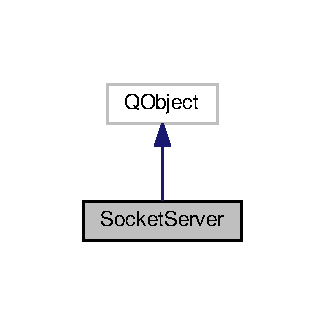
\includegraphics[width=156pt]{classSocketServer__inherit__graph}
\end{center}
\end{figure}


Collaboration diagram for Socket\+Server\+:
\nopagebreak
\begin{figure}[H]
\begin{center}
\leavevmode
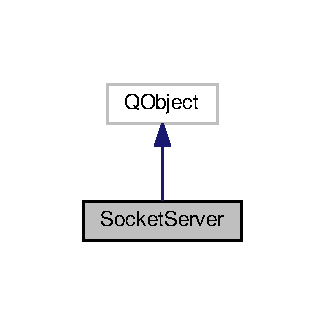
\includegraphics[width=156pt]{classSocketServer__coll__graph}
\end{center}
\end{figure}
\subsection*{Signals}
\begin{DoxyCompactItemize}
\item 
void \hyperlink{classSocketServer_a59d8051aa46795d73bd112afaa850f37}{update} ()\hypertarget{classSocketServer_a59d8051aa46795d73bd112afaa850f37}{}\label{classSocketServer_a59d8051aa46795d73bd112afaa850f37}

\begin{DoxyCompactList}\small\item\em Signal to update the gui. \end{DoxyCompactList}\end{DoxyCompactItemize}
\subsection*{Public Member Functions}
\begin{DoxyCompactItemize}
\item 
\hyperlink{classCache}{Cache} $\ast$ \hyperlink{classSocketServer_aaba9d7f97268569494b238b19c1558b5}{get\+\_\+cache} ()
\begin{DoxyCompactList}\small\item\em Return memory. \end{DoxyCompactList}\item 
\hyperlink{classMemory}{Memory} $\ast$ \hyperlink{classSocketServer_ad10dc09c0187d051829bf4073874268a}{get\+\_\+memory} ()
\begin{DoxyCompactList}\small\item\em Return memory. \end{DoxyCompactList}\item 
void \hyperlink{classSocketServer_afac9dc85dd014e6288551aa49f74f63f}{run} ()\hypertarget{classSocketServer_afac9dc85dd014e6288551aa49f74f63f}{}\label{classSocketServer_afac9dc85dd014e6288551aa49f74f63f}

\begin{DoxyCompactList}\small\item\em Run server. \end{DoxyCompactList}\item 
\hyperlink{classSocketServer_aaf00434c8b9e0cd301d9744dfea23559}{Socket\+Server} (Q\+Object $\ast$parent=0)\hypertarget{classSocketServer_aaf00434c8b9e0cd301d9744dfea23559}{}\label{classSocketServer_aaf00434c8b9e0cd301d9744dfea23559}

\begin{DoxyCompactList}\small\item\em Constructor. \end{DoxyCompactList}\item 
\hyperlink{classSocketServer_af0e595690e453ef4b8e8da174069aba9}{$\sim$\+Socket\+Server} ()\hypertarget{classSocketServer_af0e595690e453ef4b8e8da174069aba9}{}\label{classSocketServer_af0e595690e453ef4b8e8da174069aba9}

\begin{DoxyCompactList}\small\item\em Destructor. \end{DoxyCompactList}\end{DoxyCompactItemize}
\subsection*{Static Public Member Functions}
\begin{DoxyCompactItemize}
\item 
static void $\ast$ \hyperlink{classSocketServer_a66e087b1fe412328d1976957881a8f37}{check\+\_\+reference\+\_\+count} (void $\ast$obj)
\begin{DoxyCompactList}\small\item\em Check if the reference count of a node has reached 0. \end{DoxyCompactList}\item 
static \hyperlink{classSocketServer}{Socket\+Server} $\ast$ \hyperlink{classSocketServer_a9a309cddebc7b17f9788f6705fd55497}{get\+\_\+instance} ()
\begin{DoxyCompactList}\small\item\em Return a static instance of this class. \end{DoxyCompactList}\end{DoxyCompactItemize}


\subsection{Detailed Description}
The \hyperlink{classSocketServer}{Socket\+Server} class. 

\subsection{Member Function Documentation}
\index{Socket\+Server@{Socket\+Server}!check\+\_\+reference\+\_\+count@{check\+\_\+reference\+\_\+count}}
\index{check\+\_\+reference\+\_\+count@{check\+\_\+reference\+\_\+count}!Socket\+Server@{Socket\+Server}}
\subsubsection[{\texorpdfstring{check\+\_\+reference\+\_\+count(void $\ast$obj)}{check_reference_count(void *obj)}}]{\setlength{\rightskip}{0pt plus 5cm}void $\ast$ Socket\+Server\+::check\+\_\+reference\+\_\+count (
\begin{DoxyParamCaption}
\item[{void $\ast$}]{obj}
\end{DoxyParamCaption}
)\hspace{0.3cm}{\ttfamily [static]}}\hypertarget{classSocketServer_a66e087b1fe412328d1976957881a8f37}{}\label{classSocketServer_a66e087b1fe412328d1976957881a8f37}


Check if the reference count of a node has reached 0. 


\begin{DoxyParams}{Parameters}
{\em obj} & -\/ memory to check. \\
\hline
\end{DoxyParams}
\index{Socket\+Server@{Socket\+Server}!get\+\_\+cache@{get\+\_\+cache}}
\index{get\+\_\+cache@{get\+\_\+cache}!Socket\+Server@{Socket\+Server}}
\subsubsection[{\texorpdfstring{get\+\_\+cache()}{get_cache()}}]{\setlength{\rightskip}{0pt plus 5cm}{\bf Cache} $\ast$ Socket\+Server\+::get\+\_\+cache (
\begin{DoxyParamCaption}
{}
\end{DoxyParamCaption}
)}\hypertarget{classSocketServer_aaba9d7f97268569494b238b19c1558b5}{}\label{classSocketServer_aaba9d7f97268569494b238b19c1558b5}


Return memory. 

\begin{DoxyReturn}{Returns}
memory. 
\end{DoxyReturn}
\index{Socket\+Server@{Socket\+Server}!get\+\_\+instance@{get\+\_\+instance}}
\index{get\+\_\+instance@{get\+\_\+instance}!Socket\+Server@{Socket\+Server}}
\subsubsection[{\texorpdfstring{get\+\_\+instance()}{get_instance()}}]{\setlength{\rightskip}{0pt plus 5cm}{\bf Socket\+Server} $\ast$ Socket\+Server\+::get\+\_\+instance (
\begin{DoxyParamCaption}
{}
\end{DoxyParamCaption}
)\hspace{0.3cm}{\ttfamily [static]}}\hypertarget{classSocketServer_a9a309cddebc7b17f9788f6705fd55497}{}\label{classSocketServer_a9a309cddebc7b17f9788f6705fd55497}


Return a static instance of this class. 

\begin{DoxyReturn}{Returns}
static instance of this class. 
\end{DoxyReturn}
\index{Socket\+Server@{Socket\+Server}!get\+\_\+memory@{get\+\_\+memory}}
\index{get\+\_\+memory@{get\+\_\+memory}!Socket\+Server@{Socket\+Server}}
\subsubsection[{\texorpdfstring{get\+\_\+memory()}{get_memory()}}]{\setlength{\rightskip}{0pt plus 5cm}{\bf Memory} $\ast$ Socket\+Server\+::get\+\_\+memory (
\begin{DoxyParamCaption}
{}
\end{DoxyParamCaption}
)}\hypertarget{classSocketServer_ad10dc09c0187d051829bf4073874268a}{}\label{classSocketServer_ad10dc09c0187d051829bf4073874268a}


Return memory. 

\begin{DoxyReturn}{Returns}
memory. 
\end{DoxyReturn}


The documentation for this class was generated from the following files\+:\begin{DoxyCompactItemize}
\item 
socketserver.\+h\item 
socketserver.\+cpp\end{DoxyCompactItemize}

\chapter{File Documentation}
\hypertarget{cache_8h}{}\section{cache.\+h File Reference}
\label{cache_8h}\index{cache.\+h@{cache.\+h}}


Contains a set of methods for handling cache.  


{\ttfamily \#include \char`\"{}nodecache.\+h\char`\"{}}\\*
{\ttfamily \#include $<$stdexcept$>$}\\*
{\ttfamily \#include $<$string$>$}\\*
Include dependency graph for cache.\+h\+:
\nopagebreak
\begin{figure}[H]
\begin{center}
\leavevmode
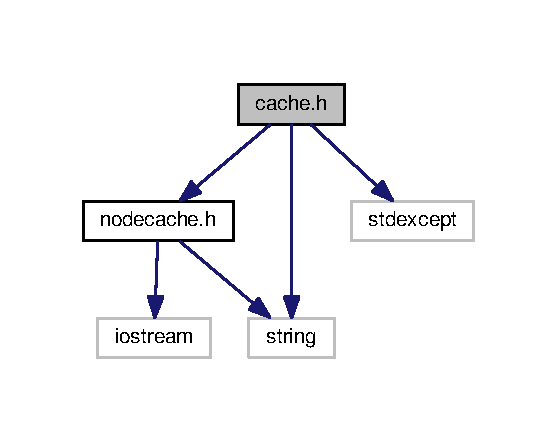
\includegraphics[width=268pt]{cache_8h__incl}
\end{center}
\end{figure}
This graph shows which files directly or indirectly include this file\+:
\nopagebreak
\begin{figure}[H]
\begin{center}
\leavevmode
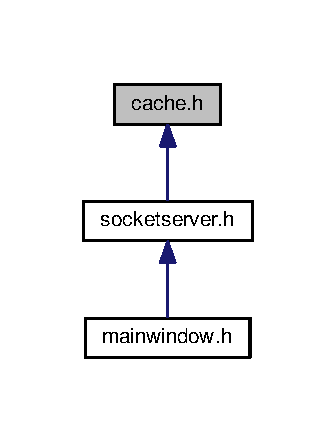
\includegraphics[width=161pt]{cache_8h__dep__incl}
\end{center}
\end{figure}
\subsection*{Classes}
\begin{DoxyCompactItemize}
\item 
class \hyperlink{classCache}{Cache}
\begin{DoxyCompactList}\small\item\em The \hyperlink{classCache}{Cache} class. \end{DoxyCompactList}\end{DoxyCompactItemize}
\subsection*{Macros}
\begin{DoxyCompactItemize}
\item 
\#define \hyperlink{cache_8h_a392fb874e547e582e9c66a08a1f23326}{M\+AX}~5
\end{DoxyCompactItemize}


\subsection{Detailed Description}
Contains a set of methods for handling cache. 

\begin{DoxyAuthor}{Author}
Erick Andres Obregon Fonseca. 
\end{DoxyAuthor}


\subsection{Macro Definition Documentation}
\index{cache.\+h@{cache.\+h}!M\+AX@{M\+AX}}
\index{M\+AX@{M\+AX}!cache.\+h@{cache.\+h}}
\subsubsection[{\texorpdfstring{M\+AX}{MAX}}]{\setlength{\rightskip}{0pt plus 5cm}\#define M\+AX~5}\hypertarget{cache_8h_a392fb874e547e582e9c66a08a1f23326}{}\label{cache_8h_a392fb874e547e582e9c66a08a1f23326}
Maximun nodes in cache 
\hypertarget{mainwindow_8h}{}\section{mainwindow.\+h File Reference}
\label{mainwindow_8h}\index{mainwindow.\+h@{mainwindow.\+h}}


\hyperlink{classMainWindow}{Main\+Window} header.  


{\ttfamily \#include $<$Q\+Main\+Window$>$}\\*
{\ttfamily \#include $<$Q\+Message\+Box$>$}\\*
{\ttfamily \#include \char`\"{}socketserver.\+h\char`\"{}}\\*
Include dependency graph for mainwindow.\+h\+:
\nopagebreak
\begin{figure}[H]
\begin{center}
\leavevmode
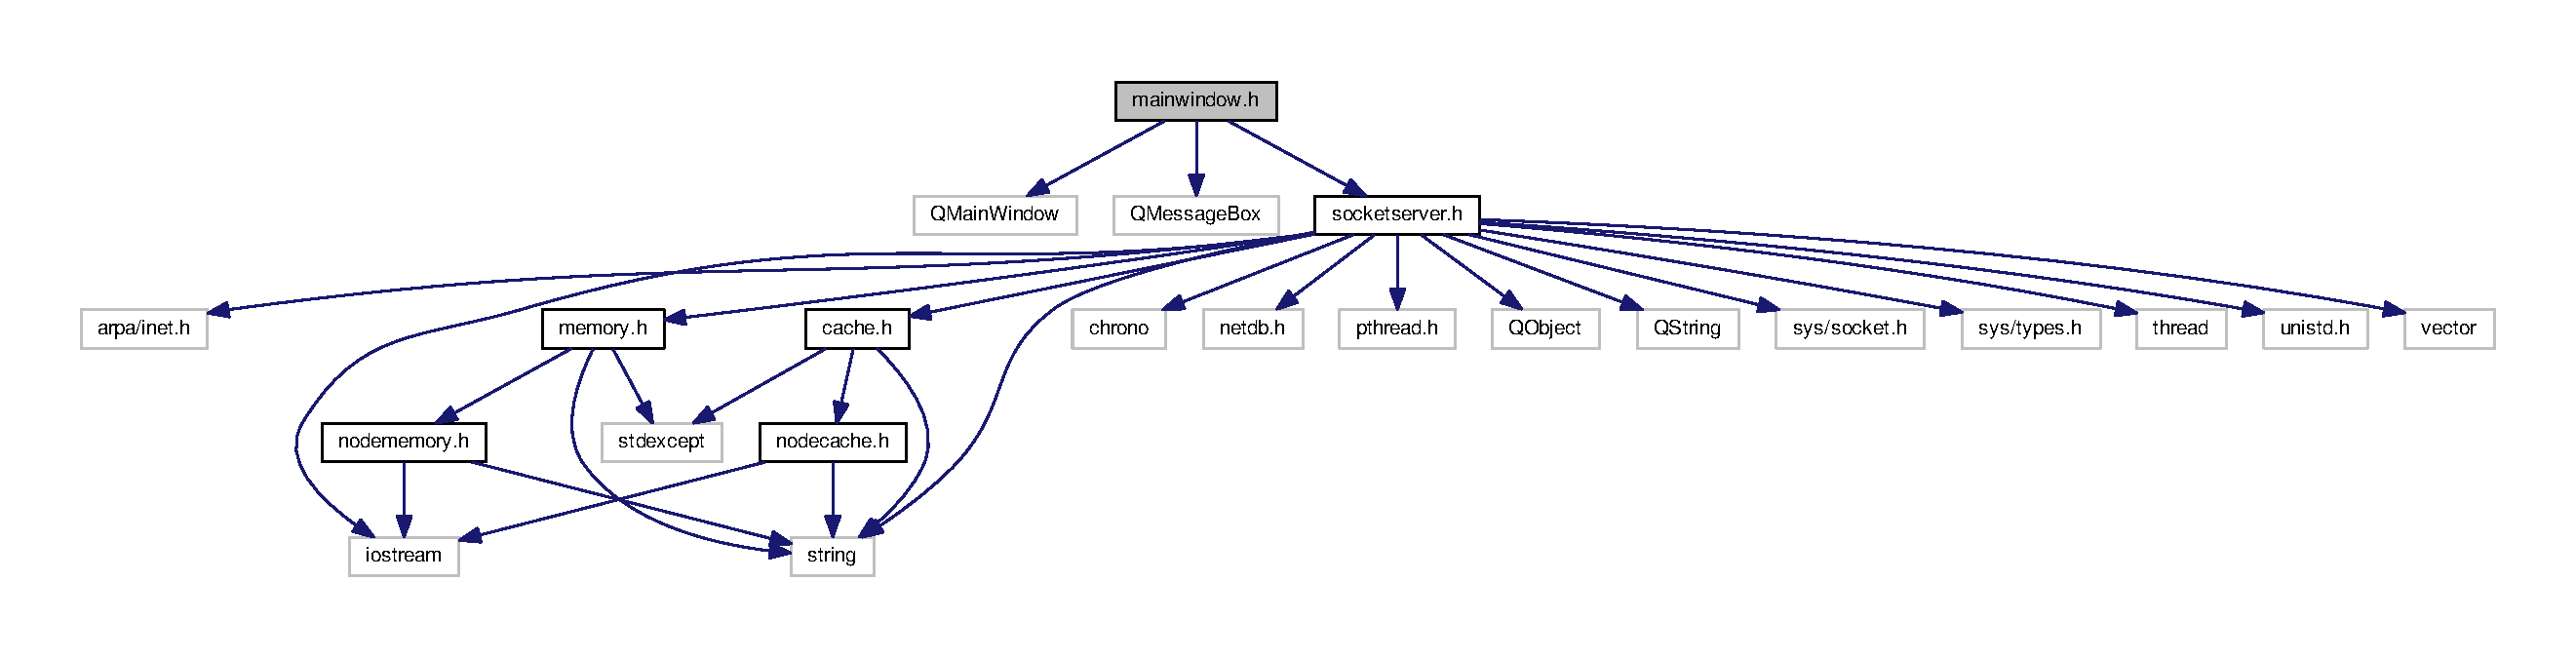
\includegraphics[width=350pt]{mainwindow_8h__incl}
\end{center}
\end{figure}
\subsection*{Classes}
\begin{DoxyCompactItemize}
\item 
class \hyperlink{classMainWindow}{Main\+Window}
\begin{DoxyCompactList}\small\item\em The \hyperlink{classMainWindow}{Main\+Window} class. \end{DoxyCompactList}\end{DoxyCompactItemize}


\subsection{Detailed Description}
\hyperlink{classMainWindow}{Main\+Window} header. 

\begin{DoxyAuthor}{Author}
Erick Andres Obregon Fonseca. 
\end{DoxyAuthor}

%--- End generated contents ---

% Index
\backmatter
\newpage
\phantomsection
\clearemptydoublepage
\addcontentsline{toc}{chapter}{Index}
\printindex

\end{document}
